\section{Exercise 3 - Buffer overflow with sign detection} \label{sec:exercise3}
Buffer overflow is historically one of the most common programming errors. It is the cause of security breaches, data corruption and program crashes. Detecting them is therefore preferred.\\\\
We start by defining a test case in the WHILE language, seen in figure \ref{code:array_example}.
\begin{figure}
  \begin{lstlisting}
program
[int A[2]]@$^1$@
[int i]@$^2$@
[i := -1]@$^3$@
while [i<3]@$^4$@ do
   [A[i] := i+1]@$^5$@
   [i := i+1]@$^6$@
od
end
 \end{lstlisting}
 \label{code:array_example}
 \caption{Code example for demonstrating buffer overflow}
\end{figure}
For the program in figure \ref{code:array_example}, the following cases should fail and thus, optimally be detected in our analysis:
\begin{description}
\item[Underflow:] Accessing an index below the base, i.e. any case where i < 0 in A[n].
\item[Overflow:] Accessing an index after the last element, i.e. any case where i > n-1 in A[n].
\end{description}

Our instance of the monotone framework becomes; 
 \begin{figure}[h]
 \centering
 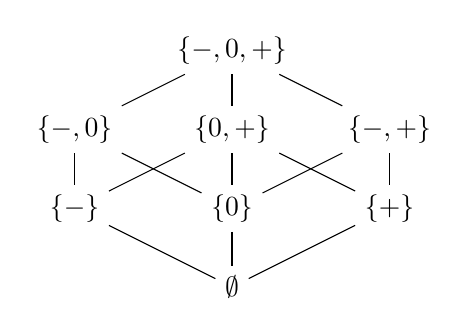
\begin{tikzpicture}
   \tikzstyle{line} = [draw, -latex'] 
   \node (nzp) at (2,3)  {$\{-,0,+\}$};
   \node (nz) at (0,2)  {$\{-,0\}$};
   \node (zp) at (2,2)  {$\{0,+\}$};
   \node (np) at (4,2)  {$\{-,+\}$};
   \node (n) at (0,1)  {$\{-\}$};
   \node (z) at (2,1)  {$\{0\}$};
   \node (p) at (4,1)  {$\{+\}$};
   \node (empty) at (2,0)  {$\emptyset$};
 
   \path [-] (nzp) edge (nz);
   \path [-] (nzp) edge  (np);
   \path [-] (nzp) edge  (zp);
 
   \path [-] (nz) edge (z);
   \path [-] (nz) edge (n);

   \path [-] (zp) edge (n);
   \path [-] (zp) edge (z);
   \path [-] (zp) edge (p);

   \path [-] (np) edge (z);
   \path [-] (np) edge (p);

   \path [-] (n) edge (empty);
   \path [-] (z) edge (empty);
   \path [-] (p) edge (empty);

 \end{tikzpicture}
  \caption{Complete lattice of sign detection instance}
 
  \label{fig:sign_detection_complete_lattice}
 \end{figure}

\begin{table}
\begin{tabular}{| l | l |}
  \hline
  Instance & $(L,\sqsubseteq,\bigsqcup, \bigsqcap, \top, \bot )$ \\
  \hline
  \hline
  Lattice  & $\{-,0,+\}$ \\
  \hline
  $\sqsubseteq$-Ordering  &  $\subseteq$ (subset ordering).\\
  \hline
  Partial ordered set    & $\mathcal{P}(\{-,0,+\}, \subseteq)$ \\
  \hline
  Least upper bound      & $\bigsqcup Y = \bigcup Y$\\
  \hline
  Greatest lower bound   & $\bigsqcap Y = \bigcap Y$\\
  \hline
  $\bot$                 & Bottom, least element : $\emptyset$\\
  \hline
  $\top$                 & Top, greatest element : $\{-,0,+\}$\\
\hline   
\end{tabular}
  \centering
  \caption{Sign detection instance}
  \label{table:sign_detection_instance}
\end{table}
This is a complete lattice, as every subset in the partial ordered set have a least upper bound and a greatest lower bound.\\
It also holds the Ascending Chain Property, because the lattice has a finite height, and will thus, eventually stabilize.\\\\
We define the flow as 
\begin{description}
  \item[Flow $F$:] flow ($S_*$) (forward analysis)
  \item[Extremal label $E$:] \{init($S_*$)\}
\end{description}

The analysis is defined as :
\begin{table}
\begin{tabular}{| l | l |}
  \hline
  Analysis$_\circ(\ell)$ & $ \bigsqcup \{$ Analysis$_\bullet (\ell') | (\ell', \ell) \in F \} \bigcup \iota_E^{\ell} $ \\
                         & where $\iota_E^{\ell} = \begin{cases} \iota & \text{if } \ell \in E \\ 
                                                                 \bot  & \text{if } \ell \notin E
                                                   \end{cases}$\\
  \hline
  Analysis$_\bullet(\ell)$ & f$_\ell$(Analysis$_\circ(\ell)$)\\
  \hline
\end{tabular}
\centering
\caption{Analysis definitions}
\end{table}

\subsection{Transfer functions}
%We define our transfer functions as
\begin{table}
\begin{tabular}{| l | l | l |}
  \hline
  \# & Statement & Function \\
  \hline
  \hline
  1 & [int x]$^\ell$ & f$_\ell^S (\widehat{\sigma}) = \widehat{\sigma}[x \mapsto {0}]$ \\
  \hline
  2 & [int A[n]]$^\ell$ & f$_\ell^S (\widehat{\sigma}) = 
     \begin{cases} 
        \widehat{\sigma}[$A[n]$ \mapsto \bot] & \text{if } \mathcal{A}_S [\![n]\!] \widehat{a} \subseteq \{-,0\} \textbf{Feedback please!} \\
        \widehat{\sigma}[$A[i]$ \mapsto {0} | \forall i \in \{0, ..., n-1 \} & \text{if } \mathcal{A}_S [\![n]\!] \widehat{a} = \{+\} \\
     \end{cases}$\\
  \hline
  3 & [x := a]$^\ell$ & f$_\ell^S (\widehat{\sigma}) = \widehat{\sigma}[x \mapsto \mathcal{A}_S[\![a]\!] \widehat{\sigma} ]$ \\
  \hline
  4 & [skip]$^\ell$ & f$_\ell^S (\widehat{\sigma}) = \widehat{\sigma}$\\
  \hline
  5 & [b]$^\ell$ & f$_\ell^S (\widehat{\sigma}) = \widehat{\sigma}$\\
  \hline
  6 & [int A[a$_1$] := a$_2$]$^\ell$ & f$_\ell^S (\widehat{\sigma}) = 
     \begin{cases} 
        \widehat{\sigma}[$A[a$_1$]$ \mapsto \bot]        & \text{if } \mathcal{A}_S [\![a_1]\!] \widehat{a} = \{-\} \\
        \widehat{\sigma}[$A[a$_1$]$ \mapsto A_I[\![a_2]\!] & \text{if }\mathcal{A}_S [\![a_1]\!] \widehat{a} \subseteq \{0,+\} \\
     \end{cases}$\\
  \hline
  7 & [read x]$^\ell$ & f$_\ell^S (\widehat{\sigma}) = [x \mapsto \mathcal{A}_S [\![n]\!] \widehat{\sigma}]$ \\
  \hline
  8 & [read A[a]]$^\ell$ & f$_\ell^S (\widehat{\sigma}) = 
     \begin{cases} 
        \widehat{\sigma}[$A[a]$ \mapsto \bot]        & \text{if } \mathcal{A}_S [\![a]\!]\widehat{\sigma} = \{-\} \\
        \widehat{\sigma}[$A[a]$ \mapsto \mathcal{A}_S[\![n]\!]\widehat{\sigma} & \text{if } \mathcal{A}_S [\![a]\!]\widehat{\sigma} = \{0,+\} \\
     \end{cases}$\\
  \hline
  9 & [write A[n]]$^\ell$ & f$_\ell^S (\widehat{\sigma}) = \widehat{\sigma}$\\
  \hline
\end{tabular}
\centering
\caption{Transfer functions for sign detection}
\label{table:sign_detection_functions}
\end{table}

$
\mathcal{A}_S [\![a]\!]: \widehat{\textbf{State}_S} \rightarrow \textbf{Sign}\\
\mathcal{A}_S [\![x]\!]\widehat{\sigma} = \widehat{\sigma} (x)\\
\mathcal{A}_S [\![n]\!]= 
   \begin{cases} 
      \{-\} & \text{ if } n < 0 \\
      \{0\} & \text{ if } n = 0 \\
      \{+\} & \text{ if } n > 0 \\
   \end{cases}\\
\mathcal{A}_S [\![a_1 \text{ op}_A a_2 ]\!] = \mathcal{A}_S [\![a_1]\!] \widehat{\sigma} \widehat{\text{ op}_A} \mathcal{A}_S [\![a_2]\!] \widehat{\sigma}, \text{where} \widehat{\text{ op}_A} : \textbf{Sign} \times \textbf{Sign} \rightarrow \textbf{Sign} \text{ is given by}:\\
\widehat{\text{ op}_A} (S_1, S_2) = \{ s_1 \text{ op}_A s_2 | s_1 \in S_1, s_2 \in S_2\}\\
\widehat{\text{ op}_A} \text {is a specific arithmatic operator from the set op}_a(\text{op}_a = \{+,-,*,/\}).
$

\begin{table}[H]
\begin{tabular}{| r | c | c | c |}
\hline
    & -           & 0 & + \\
\hline
 -  & $\{-\}$     & $\{-\}$ & $\{-,0,+\}$ \\
\hline
 0  & $\{-\}$     & $\{0\}$ & $\{+\}$ \\
\hline
 +  & $\{-,0,+\}$ & $\{+\}$ & $\{-\}$ \\
\hline
\end{tabular}
\centering
\caption{Addition effects on variable state}
\end{table}

\begin{table}[H]
\begin{tabular}{| r | c | c | c |}
\hline
    & -           & 0 & + \\
\hline
 -  & $\{-,0,+\}$ & $\{-\}$ & $\{-\}$ \\
\hline
 0  & $\{-\}$     & $\{0\}$ & $\{-\}$ \\
\hline
 +  & $\{+\}$     & $\{+\}$ & $\{-,0,+\}$ \\
\hline
\end{tabular}
\centering
\caption{Subtraction effects on variable state}
\end{table}

\begin{table}[H]
\begin{tabular}{| r | c | c | c |}
\hline
    & -           & 0 & + \\
\hline
 -  & $\{+\}$ & $\{0\}$ & $\{-\}$ \\
\hline
 0  & $\{0\}$ & $\{0\}$ & $\{0\}$ \\
\hline
 +  & $\{-\}$ & $\{0\}$ & $\{+\}$ \\
\hline
\end{tabular}
\centering
\caption{Multiplication effects on variable state}
\end{table}

\begin{table}[H]
\begin{tabular}{| r | c | c | c |}
\hline
    & -           & 0 & + \\
\hline
 -  & $\{+\}$ & $\emptyset$ & $\{-\}$ \\
\hline
 0  & $\{0\}$ & $\emptyset$ & $\{0\}$ \\
\hline
 +  & $\{-\}$ & $\emptyset$ & $\{+\}$ \\
\hline
\end{tabular}
\centering
\caption{Division effects on variable state}
\end{table}


\subsection{Lower bound detection}
Check for an assignment which includes an operation with an array, that the sign of the array is not $\emptyset$. If so, we know that the index parameter is invalid according to the lower bounds.

\subsection{Constraints}
\begin{table}[H]
\begin{tabular}{| l | l |}
\hline
A$_\circ (1) = \iota \{\text{init}(S_*) \} $ & A$_\bullet(1) = \text{f}_{\text{int A[2]}} (\text{A}_\circ (1))$ \\
\hline
A$_\circ (2) =$A$_\bullet(1) $ & A$_\bullet(2) = \text{f}_{\text{int i}} (\text{A}_\circ (2))$ \\
\hline
A$_\circ (3) = $A$_\bullet(2)$ & A$_\bullet(3) = \text{f}_{\text{i := -1}} (\text{A}_\circ (3))$  \\
\hline
A$_\circ (4) = $A$_\bullet(3) \bigcup $A$_\bullet(6) $ & A$_\bullet(4) = \text{f}_{\text{i < 3}} (\text{A}_\circ (4))$ \\
\hline
A$_\circ (5) = $A$_\bullet(4)$ & A$_\bullet(5) = \text{f}_{\text{A[i] := i + 1}} (\text{A}_\circ (5))$ \\
\hline
A$_\circ (6) = $A$_\bullet(5)$ & A$_\bullet(6) = \text{f}_{\text{i := i + 1}} (\text{A}_\circ (6))$ \\

\hline
\end{tabular}
\centering
\end{table}

\begin{table}[H]
\begin{tabular}{| r | c | c | c |}
\hline
A$_\bullet (\cdot) $ & A[0]        & A[1]        & i \\
\hline
1                    & $\{0\}$     & $\{0\} $    & $\emptyset$ \\
2                    & $\{0\}$     & $\{0\} $    & $\{0\}$ \\
3                    & $\{0\}$     & $\{0\} $    & $\{-\}$ \\
4                    & $\{-,0,+\}$ & $\{-,0,+\}$ & $\{-,0,+\}$ \\
5                    & $\{-,0,+\}$ & $\{-,0,+\}$ & $\{-,0,+\}$ \\
6                    & $\{-,0,+\}$ & $\{-,0,+\}$ & $\{-,0,+\}$ \\
\hline
\end{tabular}
\centering
\end{table}
